\documentclass[a4paper,12pt]{paper}

\usepackage{mycommands}

% Worked-example layout: boxed problem statement followed by a solution.
\newcounter{example}
\renewenvironment{example}[1]{%  % the paper class already defines "example"
  \refstepcounter{example}%
  \begin{mdframed}[linewidth=1pt,innertopmargin=6pt,innerbottommargin=6pt]%
  \noindent\textbf{Example \theexample: #1.}\ }{%
  \end{mdframed}}
\newenvironment{solution}{\par\noindent\textbf{Solution.}\ }{\par\medskip}

\title{Worked examples for Lecture 23: Mode splitting and coupling}
\author{David Al-Attar \\ Michaelmas Term, \the\year}

\begin{document}

\maketitle

\noindent These examples accompany Lecture~23. They are intended as practice in the concrete
calculations that underlie the lecture, and are less demanding than the questions on the
problem sets. Example~1 works through the toroidal mode problem for a homogeneous earth
model in the detail referred to in the lecture summary. Numerical results were checked with
the scripts in the \texttt{python} directory.

%-----------------------------------------------------------------------------------------
\begin{example}{Toroidal modes of a homogeneous sphere}
In the lecture it was stated that, within an entirely solid and spherically symmetric earth
model of radius $b$, the eigenvalue problem for a toroidal mode of degree $l$ reduces to
\begin{align}
&-\omega^{2}\int_{0}^{b}\rho W'^{*}Wr^{2}\dd r
+\int_{0}^{b}\mu\left(r\frac{\ddns W'^{*}}{\ddns r}-W'^{*}\right)\left(r\frac{\ddns W}{\ddns r}-W\right)\dd r\nonumber\\
&+(\zeta^{2}-2)\int_{0}^{b}\mu W'^{*}W\dd r=0,
\label{eq:1}
\end{align}
which is to hold for all test functions $W'$, where $\zeta^{2}=l(l+1)$ and $W$ is the radial
eigenfunction. (i)~By integrating by parts, show that eq.~(\ref{eq:1}) is equivalent to an
ordinary differential equation of Sturm--Liouville type for $W$ on $0<r<b$ together with a
boundary condition at $r=b$, and interpret this boundary condition physically. (ii)~Show that
when $\rho$ and $\mu$ are constant the solution regular at the centre is $W(r)=j_{l}(kr)$,
with $k=\omega/\beta$, $\beta=\sqrt{\mu/\rho}$, and $j_{l}$ the spherical Bessel function of
the first kind, and obtain the equation that determines the eigenfrequencies. (iii)~Solve this
equation numerically for $l=2$ and $l=3$, tabulating the periods of the first three overtones
for a homogeneous sphere with $b=6371\,\mathrm{km}$ and $\beta=6.3\,\mathrm{km\,s^{-1}}$, and
compare the period of ${}_{0}T_{2}$ with the observed value of $44.2\,\mathrm{min}$.
\end{example}

\begin{solution}
Throughout this example there is no time dependence, and so we use a dot to denote
$\ddns/\ddns r$; as in the lecture, $W'$ is the test function and not a derivative.

\medskip
\noindent\textit{(i) The radial equation and its boundary condition.}
Expanding the product in the second integral of eq.~(\ref{eq:1}) gives
\begin{equation}
\mu\left(r\dot{W}'^{*}-W'^{*}\right)\left(r\dot{W}-W\right)
=\mu r^{2}\dot{W}'^{*}\dot{W}-\mu r\dot{W}'^{*}W-\mu rW'^{*}\dot{W}+\mu W'^{*}W,
\label{eq:2}
\end{equation}
and we integrate by parts the two terms that contain the derivative of the test function,
\begin{align}
\int_{0}^{b}\mu r^{2}\dot{W}'^{*}\dot{W}\dd r&=\left[\mu r^{2}W'^{*}\dot{W}\right]_{0}^{b}
-\int_{0}^{b}W'^{*}\frac{\ddns}{\ddns r}\left(\mu r^{2}\dot{W}\right)\dd r,\label{eq:3}\\
-\int_{0}^{b}\mu r\dot{W}'^{*}W\dd r&=-\left[\mu rW'^{*}W\right]_{0}^{b}
+\int_{0}^{b}W'^{*}\frac{\ddns}{\ddns r}\left(\mu rW\right)\dd r.\label{eq:4}
\end{align}
The boundary terms at $r=0$ vanish so long as $W$, $\dot{W}$ and $W'$ remain bounded at the
centre, which we assume. Since $\frac{\ddns}{\ddns r}(\mu rW)=r\dot{\mu}W+\mu W+\mu r\dot{W}$,
the term $\mu r\dot{W}$ cancels against the third term on the right of eq.~(\ref{eq:2}), and
collecting everything eq.~(\ref{eq:1}) becomes
\begin{equation}
\int_{0}^{b}W'^{*}\left[-\frac{\ddns}{\ddns r}\left(\mu r^{2}\dot{W}\right)
+\left(\zeta^{2}\mu+r\dot{\mu}\right)W-\omega^{2}\rho r^{2}W\right]\dd r
+b^{2}\,W'^{*}(b)\,T(b)=0,
\label{eq:5}
\end{equation}
where we have introduced the function
\begin{equation}
T(r)=\mu\left(\dot{W}-\frac{W}{r}\right)=\mu r\frac{\ddns}{\ddns r}\left(\frac{W}{r}\right).
\label{eq:6}
\end{equation}
Eq.~(\ref{eq:5}) must hold for every test function. Considering first those that vanish at
$r=b$ but are otherwise arbitrary, the square bracket must vanish for $0<r<b$, and so $W$
satisfies
\begin{equation}
\frac{\ddns}{\ddns r}\left(\mu r^{2}\frac{\ddns W}{\ddns r}\right)
-\left(\zeta^{2}\mu+r\frac{\ddns\mu}{\ddns r}\right)W+\omega^{2}\rho r^{2}W=0.
\label{eq:7}
\end{equation}
Given eq.~(\ref{eq:7}), the integral in eq.~(\ref{eq:5}) vanishes identically, and what
remains must vanish for arbitrary values of $W'(b)$. Hence we also require
\begin{equation}
T(b)=\mu\left(\frac{\ddns W}{\ddns r}-\frac{W}{r}\right)\bigg|_{r=b}=0.
\label{eq:8}
\end{equation}
Conversely, if $W$ satisfies eqs.~(\ref{eq:7}) and (\ref{eq:8}) then eq.~(\ref{eq:5}), and
hence eq.~(\ref{eq:1}), holds for every test function; the two formulations are equivalent.

Eq.~(\ref{eq:7}) has the Sturm--Liouville form $\frac{\ddns}{\ddns r}(p\dot{W})-qW+\lambda wW=0$ with
$p=\mu r^{2}$, $q=\zeta^{2}\mu+r\dot{\mu}$, weight $w=\rho r^{2}$, and eigenvalue
$\lambda=\omega^{2}$. Standard theory for such problems then gives directly what the lecture
stated in general: the squared eigenfrequencies are real, eigenfunctions with distinct
eigenfrequencies are orthogonal with respect to $\int_{0}^{b}\rho W_{n}W_{n'}r^{2}\dd r$, which is
just the kinetic energy form restricted to toroidal modes of degree $l$, and there is a
countable infinity of eigenvalues accumulating at infinity, labelled by the overtone number
$n=0,1,2,\dots$. The boundary condition in eq.~(\ref{eq:8}) was not imposed but emerged from
the weak form; it is a \textit{natural} boundary condition. Its physical meaning follows from
computing the traction on a spherical surface. For a toroidal displacement
$\mathbf{s}=W\mathbf{C}_{lm}$ the radial component vanishes, and the shear strains in an
isotropic model give $\sigma_{r\theta}=\mu(\dot{W}-W/r)C_{\theta}$ and
$\sigma_{r\varphi}=\mu(\dot{W}-W/r)C_{\varphi}$, so that the traction acting on the surface
$r=\mathrm{const}$ is $T(r)\mathbf{C}_{lm}$. Eq.~(\ref{eq:8}) is therefore precisely the
traction-free condition at the free surface, as was to be expected from the discussion in
Lecture~22 of how boundary conditions are built into the weak form. It is also worth noting
the identity $r\dot{W}-W=r^{2}\frac{\ddns}{\ddns r}(W/r)$: the first potential energy
term in eq.~(\ref{eq:1}) vanishes for $W\propto r$, which for $l=1$ is a rigid rotation, and
we return to this point below.

\medskip
\noindent\textit{(ii) The homogeneous sphere.}
If $\rho$ and $\mu$ are constant then $\dot{\mu}=0$, and dividing eq.~(\ref{eq:7}) by
$\mu r^{2}$ we obtain
\begin{equation}
\frac{\ddns^{2}W}{\ddns r^{2}}+\frac{2}{r}\frac{\ddns W}{\ddns r}
+\left[k^{2}-\frac{l(l+1)}{r^{2}}\right]W=0,\quad k=\frac{\omega}{\beta},
\quad \beta=\sqrt{\frac{\mu}{\rho}}.
\label{eq:9}
\end{equation}
In terms of $x=kr$ this is the spherical Bessel equation of order $l$, with general solution
$W=Aj_{l}(kr)+By_{l}(kr)$. Near the centre, trying $W\propto r^{\alpha}$ in eq.~(\ref{eq:9})
gives at leading order $\alpha(\alpha+1)=l(l+1)$, so that $\alpha=l$ or $\alpha=-(l+1)$; these
are the behaviours $j_{l}(x)\sim x^{l}/(2l+1)!!$ and $y_{l}(x)\sim-(2l-1)!!/x^{l+1}$ of the
two solutions. The second is unbounded, and would give an infinite kinetic energy since
$\int_{0}\rho W^{2}r^{2}\dd r$ then behaves like $\int_{0}r^{-2l}\dd r$ for $l\ge1$. Hence
$B=0$, and up to an arbitrary amplitude
\begin{equation}
W(r)=j_{l}(kr).
\label{eq:10}
\end{equation}
The eigenfrequencies follow from the traction-free condition in eq.~(\ref{eq:8}), which reads
$\mu[kj_{l}'(kb)-j_{l}(kb)/b]=0$. Writing $x=kb=\omega b/\beta$, this is
\begin{equation}
xj_{l}'(x)=j_{l}(x),\quad\text{or equivalently}\quad
\frac{\ddns}{\ddns x}\left[\frac{j_{l}(x)}{x}\right]=0 .
\label{eq:11}
\end{equation}
Using the recurrence relation $j_{l}'(x)=\frac{l}{x}j_{l}(x)-j_{l+1}(x)$ we can also write the
frequency equation as
\begin{equation}
(l-1)j_{l}(x)=xj_{l+1}(x).
\label{eq:12}
\end{equation}
For each degree this transcendental equation has a countable infinity of positive roots
$x_{0}<x_{1}<x_{2}<\cdots$, and the mode ${}_{n}T_{l}$ has eigenfrequency and period
\begin{equation}
\omega=\frac{\beta x_{n}}{b},\quad \mathcal{T}=\frac{2\pi b}{\beta x_{n}}.
\label{eq:13}
\end{equation}
For $l=2$, inserting $j_{1}(x)=\sin x/x^{2}-\cos x/x$ and
$j_{2}(x)=(3/x^{3}-1/x)\sin x-3\cos x/x^{2}$ into eq.~(\ref{eq:11}) and clearing
denominators gives the explicit form
\begin{equation}
\tan x=\frac{x(x^{2}-12)}{5x^{2}-12},
\label{eq:14}
\end{equation}
which shows clearly that the roots must be found numerically. For large $x$ we have
$j_{l}(x)\approx\sin(x-l\pi/2)/x$, so eq.~(\ref{eq:11}) becomes
$\tan(x-l\pi/2)\approx x/2$ and successive roots are separated by approximately $\pi$: the
overtones of a given degree become equally spaced in frequency, with spacing
$\Delta f=\beta/2b$, which is the inverse of the two-way travel time of an S-wave across a
diameter of the sphere. Finally, we note the special case $l=1$, for which eq.~(\ref{eq:12})
reduces to $j_{2}(kb)=0$. This has the root $k=0$, corresponding to $\omega=0$ and, from the
small-argument form of $j_{1}$, to $W\propto r$. Since $r\mathbf{C}_{1m}$ is a rigid rotation
(see Example~5), this is one of the trivial zero-frequency modes discussed in Lecture~22, and
there is no fundamental toroidal mode of degree one.

\medskip
\noindent\textit{(iii) Numerical results.}
The roots of eq.~(\ref{eq:11}) were found by locating sign changes of $xj_{l}'(x)-j_{l}(x)$
on a fine grid and refining each by bisection, with $j_{l}$ and $j_{l}'$ evaluated using
\texttt{scipy.special.spherical\_jn}. With $b=6371\,\mathrm{km}$ and
$\beta=6.3\,\mathrm{km\,s^{-1}}$ we obtain the values in the table below. The shear wave
speed chosen is a crude average over the mantle, whose values in PREM range from about
$4.5\,\mathrm{km\,s^{-1}}$ beneath the crust to about $7.3\,\mathrm{km\,s^{-1}}$ at its base.

\begin{center}
\begin{tabular}{lccc}
\hline
mode & $x_{n}=kb$ & $f=\omega/2\pi$ (mHz) & period (min)\\
\hline
${}_{0}T_{2}$ & 2.5011 & 0.3936 & 42.3\\
${}_{1}T_{2}$ & 7.1360 & 1.1231 & 14.8\\
${}_{2}T_{2}$ & 10.5146 & 1.6548 & 10.1\\
${}_{0}T_{3}$ & 3.8647 & 0.6082 & 27.4\\
${}_{1}T_{3}$ & 8.4449 & 1.3291 & 12.5\\
${}_{2}T_{3}$ & 11.8817 & 1.8700 & 8.9\\
\hline
\end{tabular}
\end{center}

\noindent The predicted period of ${}_{0}T_{2}$ is $42.3\,\mathrm{min}$, about $4\%$ shorter
than the observed $44.2\,\mathrm{min}$ ($f=0.377\,\mathrm{mHz}$); a shear wave speed of
$6.03\,\mathrm{km\,s^{-1}}$ would reproduce the observation exactly. Given how crude the model
is, this agreement is better than we have any right to expect, and it is partly fortuitous.
The Earth has a fluid outer core in which toroidal motion cannot be sustained, so the real
mode is confined to the mantle, a shell occupying only the outer $45\%$ of the radius; this
stiffening of the problem raises the frequency. Against this, the low shear wave speeds of
the upper mantle, where the fundamental mode has its largest displacements
(Fig.~\ref{fig:1}), lower the frequency, and the two effects roughly compensate. For
${}_{0}T_{3}$ the model gives $27.4\,\mathrm{min}$ against an observed period of about
$28.4\,\mathrm{min}$. Fig.~\ref{fig:1} shows the radial eigenfunctions of the three lowest
$l=2$ modes. The number of interior zeros of $W$ equals the overtone number $n$, as the
oscillation theorem for Sturm--Liouville problems guarantees, and the higher overtones
oscillate increasingly rapidly with radius while the fundamental mode is smooth and largest at
the surface.

\begin{figure}[ht]
    \centering
    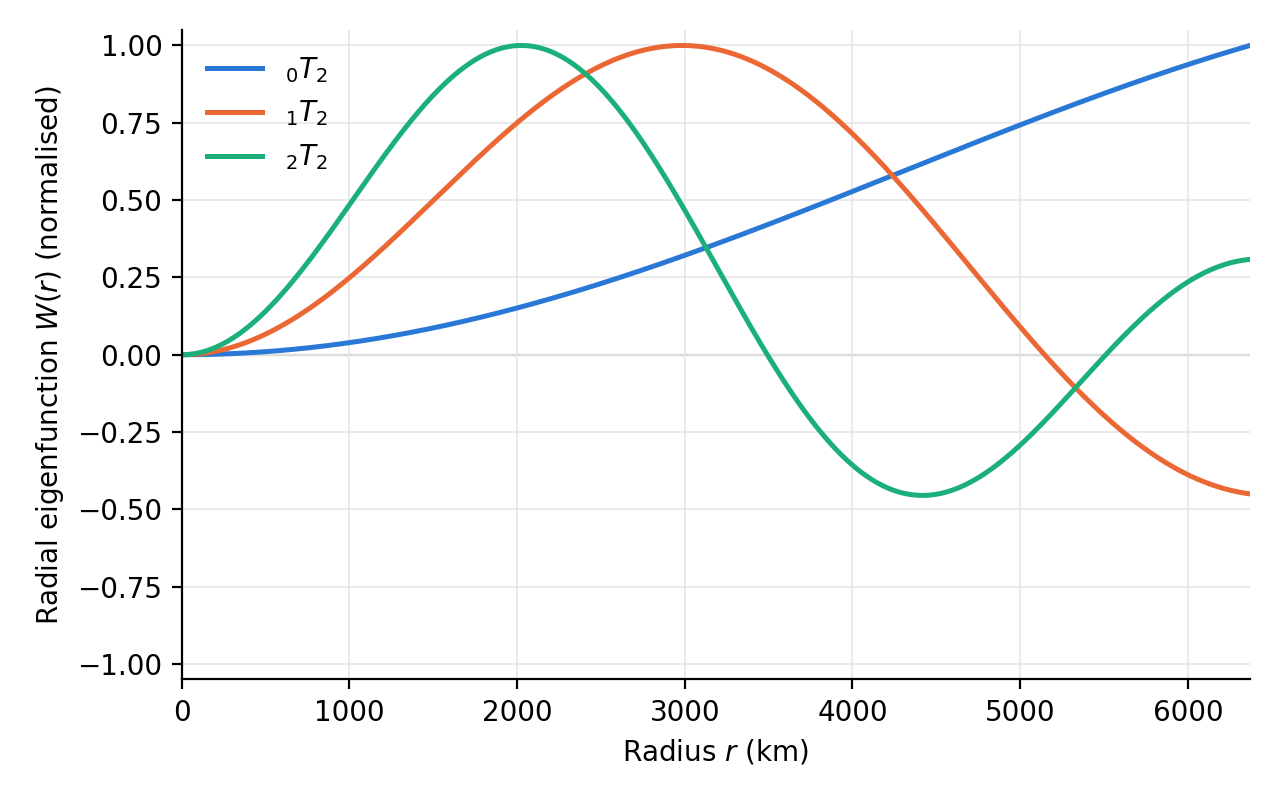
\includegraphics[width=0.7\textwidth]{figures_ex/ex12_toroidal.png}
    \caption{Radial eigenfunctions $W(r)=j_{2}(x_{n}r/b)$ of the toroidal modes
    ${}_{0}T_{2}$, ${}_{1}T_{2}$ and ${}_{2}T_{2}$ of a homogeneous sphere with
    $b=6371\,\mathrm{km}$, each normalised to unit maximum absolute value. The mode
    ${}_{n}T_{2}$ has $n$ zeros in the interior, and all three satisfy the traction-free
    condition $\dot{W}=W/b$ at the surface.}
    \label{fig:1}
\end{figure}

This example illustrates how the abstract eigenvalue problem of the lecture becomes a
concrete boundary value problem once spherical symmetry is used, and that even the simplest
conceivable earth model predicts the gravest toroidal period to within a few per cent.
\end{solution}

%-----------------------------------------------------------------------------------------
\begin{example}{The diagonal sum rule for a degree-one multiplet}
For a multiplet with $l=1$ the first-order splitting problem of the lecture is the
$3\times3$ Hermitian eigenvalue problem $\sum_{m}M_{m'm}a_{m}=\delta\omega\,a_{m'}$, with
$m,m'\in\{-1,0,1\}$ and
\begin{equation*}
M_{m'm}=\frac{1}{2\omega_{k}}\left[-\omega_{k}^{2}\langle km'|P_{1}|km\rangle
+\ii\omega_{k}\langle km'|W|km\rangle+\langle km'|H_{1}|km\rangle\right].
\end{equation*}
Suppose that, ordering the indices as $m=-1,0,1$, this splitting matrix is
\begin{equation*}
M=\begin{pmatrix}-\Delta&\epsilon&0\\ \epsilon&0&\epsilon\\ 0&\epsilon&\Delta\end{pmatrix},
\end{equation*}
with $\Delta>0$ and $\epsilon$ real, the diagonal part representing splitting by rotation
(see Example~3) and the off-diagonal part a small contribution from lateral heterogeneity.
(i)~Find the three singlet eigenfrequency perturbations and verify that the arithmetic mean
of the split eigenfrequencies equals the degenerate eigenfrequency $\omega_{k}$. (ii)~Find
the corresponding coefficient vectors $a_{m}$, verify that they are orthonormal, and explain
what this implies for the zeroth-order eigenfunctions $\mathbf{s}=\sum_{m}a_{m}|km\rangle$.
(iii)~Explain why the conclusion of part (i) holds for any Hermitian splitting matrix with
zero trace.
\end{example}

\begin{solution}
\textit{(i)} The eigenvalues $\delta\omega$ are the roots of $\det(M-\delta\omega I)=0$.
Expanding along the first row,
\begin{align}
\det(M-\delta\omega I)&=(-\Delta-\delta\omega)\left[-\delta\omega(\Delta-\delta\omega)-\epsilon^{2}\right]
-\epsilon\left[\epsilon(\Delta-\delta\omega)\right]\nonumber\\
&=-\delta\omega\left(\delta\omega^{2}-\Delta^{2}-2\epsilon^{2}\right),
\label{eq:15}
\end{align}
where the terms in $\Delta\epsilon^{2}$ cancel. The singlet perturbations are therefore
\begin{equation}
\delta\omega=-\Lambda,\quad 0,\quad +\Lambda,\qquad \Lambda=\sqrt{\Delta^{2}+2\epsilon^{2}},
\label{eq:16}
\end{equation}
and the split eigenfrequencies are $\omega_{k}-\Lambda$, $\omega_{k}$ and $\omega_{k}+\Lambda$,
whose arithmetic mean is $\omega_{k}$. Rotation alone ($\epsilon=0$) gives three equally spaced
lines with spacing $\Delta$; the heterogeneity leaves the central singlet where it is but
pushes the outer two further apart, since $\Lambda>\Delta$. As an illustration, if
$\Delta/2\pi=3\,\mu\mathrm{Hz}$ and $\epsilon/2\pi=2\,\mu\mathrm{Hz}$ then
$\Lambda/2\pi=\sqrt{17}\,\mu\mathrm{Hz}=4.12\,\mu\mathrm{Hz}$.

\medskip
\noindent\textit{(ii)} For $\delta\omega=0$ the equations $M\mathbf{a}=0$ give
$a_{0}=(\Delta/\epsilon)a_{-1}$ and $a_{1}=-a_{-1}$, while for $\delta\omega=\pm\Lambda$ the
first and third rows give $a_{0}=(\Delta\pm\Lambda)a_{-1}/\epsilon$ and
$a_{0}=(\Delta\mp\Lambda)a_{1}/\epsilon$. Using $\Lambda^{2}-\Delta^{2}=2\epsilon^{2}$ to
simplify, and normalising, we find
\begin{equation}
\mathbf{a}^{(0)}=\frac{1}{\Lambda}\begin{pmatrix}\epsilon\\ \Delta\\ -\epsilon\end{pmatrix},\quad
\mathbf{a}^{(\pm)}=\frac{1}{2\Lambda}\begin{pmatrix}\Lambda\mp\Delta\\ \pm2\epsilon\\ \Lambda\pm\Delta\end{pmatrix}.
\label{eq:17}
\end{equation}
It is readily checked that $M\mathbf{a}^{(\pm)}=\pm\Lambda\mathbf{a}^{(\pm)}$; for example the
middle row of $M\mathbf{a}^{(+)}$ is $\epsilon(\Lambda-\Delta)+\epsilon(\Lambda+\Delta)=2\epsilon\Lambda$,
which is $\Lambda$ times the middle entry of $\mathbf{a}^{(+)}$. For the norms,
$\|\mathbf{a}^{(0)}\|^{2}=(\Delta^{2}+2\epsilon^{2})/\Lambda^{2}=1$ and
\begin{equation}
\|\mathbf{a}^{(\pm)}\|^{2}=\frac{(\Lambda\mp\Delta)^{2}+4\epsilon^{2}+(\Lambda\pm\Delta)^{2}}{4\Lambda^{2}}
=\frac{2\Lambda^{2}+2\Delta^{2}+4\epsilon^{2}}{4\Lambda^{2}}=1,
\label{eq:18}
\end{equation}
while for the inner products
\begin{align}
\mathbf{a}^{(+)}\cdot\mathbf{a}^{(-)}&=\frac{(\Lambda^{2}-\Delta^{2})-4\epsilon^{2}+(\Lambda^{2}-\Delta^{2})}{4\Lambda^{2}}=0,\nonumber\\
\mathbf{a}^{(0)}\cdot\mathbf{a}^{(\pm)}&=\frac{\epsilon(\Lambda\mp\Delta)\pm2\epsilon\Delta-\epsilon(\Lambda\pm\Delta)}{2\Lambda^{2}}=0 .
\label{eq:19}
\end{align}
The three coefficient vectors are thus orthonormal, as the eigenvectors of a Hermitian matrix
with distinct eigenvalues must be. Because the singlets satisfy
$\langle km|P_{0}|km'\rangle=\delta_{mm'}$, the zeroth-order eigenfunctions
$\mathbf{s}^{(j)}=\sum_{m}a^{(j)}_{m}|km\rangle$ obey
\begin{equation}
\langle\mathbf{s}^{(j)}|P_{0}|\mathbf{s}^{(j')}\rangle=\sum_{m}a_{m}^{(j)*}a_{m}^{(j')}=\delta_{jj'},
\label{eq:20}
\end{equation}
so they are orthonormal with respect to the kinetic energy form, exactly as Lecture~22
requires of eigenfunctions with distinct eigenfrequencies. Note that for $\epsilon\ne0$ each
of these eigenfunctions is a mixture of all three singlets; the heterogeneity has selected a
particular orthonormal basis of the degenerate eigenspace, and it is this basis, not the
original singlets, that the perturbed eigenfunctions approach as the perturbation is
switched off. As $\epsilon\to0$ we recover $\mathbf{a}^{(\pm)}\to(0,0,1)$ and $(1,0,0)$, the
singlets themselves.

\medskip
\noindent\textit{(iii)} For any Hermitian matrix we can write $M=U\,\mathrm{diag}(\delta\omega_{1},\dots,\delta\omega_{2l+1})\,U^{\dagger}$
with $U$ unitary, and the cyclic property of the trace gives
$\mathrm{tr}\,M=\mathrm{tr}\,(\mathrm{diag}(\delta\omega_{j})U^{\dagger}U)=\sum_{j}\delta\omega_{j}$.
Equivalently, the coefficient of $\delta\omega^{2l}$ in the characteristic polynomial is
$-\mathrm{tr}\,M$ up to sign, as eq.~(\ref{eq:15}) illustrates. Hence if $\mathrm{tr}\,M=0$
the singlet perturbations sum to zero, and the mean of the $2l+1$ split eigenfrequencies is
$\omega_{k}$. The content of the diagonal sum rule of the lecture is the statement, following
from the selection rules for the matrix elements, that the trace does vanish for splitting by
rotation and by lateral heterogeneity, so that averaging the observed singlet frequencies
recovers the eigenfrequency of the spherically averaged Earth.
\end{solution}

%-----------------------------------------------------------------------------------------
\begin{example}{Rotational splitting is linear in $m$}
Within a multiplet $|km\rangle$, $-l\le m\le l$, of a spherically symmetric earth model it can
be shown, using the conventions of the lecture, that the matrix elements of the Coriolis form
are
\begin{equation*}
\langle km'|W|km\rangle=-2\ii\Omega\beta_{k}m\,\delta_{mm'},
\end{equation*}
where $\Omega$ is the angular rate of rotation and $\beta_{k}$ is a dimensionless constant,
the \textbf{splitting parameter}, that depends on the radial eigenfunctions of the multiplet.
Take this result as given. (i)~Check that it is consistent with the anti-self-adjointness of
the Coriolis form. (ii)~Neglecting the perturbations $P_{1}$ and $H_{1}$ (which for a rotating
earth model describe the ellipticity of figure and the centrifugal potential), solve the
first-order Hermitian eigenvalue problem of the lecture, and show that
$\delta\omega_{m}=m\Omega\beta_{k}$, so that the multiplet splits into $2l+1$ equally spaced
lines. (iii)~For ${}_{0}S_{2}$, with degenerate frequency $f_{k}=0.3094\,\mathrm{mHz}$ and
$\beta_{k}\approx0.40$, give the spacing of adjacent singlets and the total width of the
multiplet in $\mu\mathrm{Hz}$, and comment on the length of record required to resolve the
singlets.
\end{example}

\begin{solution}
\textit{(i)} In Lecture~22 we showed that $\langle\mathbf{w}|W|\mathbf{u}\rangle=-\langle\mathbf{u}|W|\mathbf{w}\rangle^{*}$.
Applied to the singlets this requires $\langle km'|W|km\rangle=-\langle km|W|km'\rangle^{*}$.
With the stated matrix elements the right-hand side is
$-(-2\ii\Omega\beta_{k}m'\delta_{m'm})^{*}=-2\ii\Omega\beta_{k}m'\delta_{mm'}$, which equals the
left-hand side because the Kronecker delta forces $m'=m$. In particular the diagonal elements
$\langle km|W|km\rangle$ are purely imaginary, as anti-self-adjointness demands. They are also
odd in $m$: the singlets $\pm m$ correspond to patterns $\ee^{\ii(\pm m\varphi+\omega t)}$
travelling in opposite directions around the rotation axis, and the Coriolis force acts on
them with opposite sign.

\medskip
\noindent\textit{(ii)} Dropping $P_{1}$ and $H_{1}$, the first-order eigenvalue problem of
the lecture reduces to
\begin{equation}
\frac{1}{2\omega_{k}}\sum_{m=-l}^{l}\ii\omega_{k}\langle km'|W|km\rangle a_{m}=\delta\omega\,a_{m'}.
\label{eq:21}
\end{equation}
Inserting the matrix elements, the sum collapses to the single term $m=m'$, and
\begin{equation}
\frac{\ii}{2}\left(-2\ii\Omega\beta_{k}m'\right)a_{m'}=\Omega\beta_{k}m'\,a_{m'}=\delta\omega\,a_{m'},
\quad -l\le m'\le l .
\label{eq:22}
\end{equation}
The splitting matrix is thus already diagonal, $M=\Omega\beta_{k}\,\mathrm{diag}(-l,\dots,l)$,
with real entries, as the diagonal of a Hermitian matrix must be. Its eigenvalues and eigenvectors can be read off: for each
$m$,
\begin{equation}
\delta\omega_{m}=m\Omega\beta_{k},\quad a_{m'}=\delta_{m'm},
\label{eq:23}
\end{equation}
so the zeroth-order eigenfunctions are the singlets $|km\rangle$ themselves, and the perturbed
eigenfrequencies are
\begin{equation}
\omega_{m}=\omega_{k}+m\Omega\beta_{k},\quad m=-l,\dots,l .
\label{eq:24}
\end{equation}
The multiplet splits into $2l+1$ lines, equally spaced by $\Omega\beta_{k}$ and placed
symmetrically about $\omega_{k}$, which is the direct analogue of the normal Zeeman effect,
$\delta E=m\mu_{B}B$, for an atom in a magnetic field. The shifts sum to
$\Omega\beta_{k}\sum_{m}m=0$, in accordance with the diagonal sum rule. The result holds to
first order in $\Omega$; the neglected terms $P_{1}$ and $H_{1}$ add a contribution that is
even in $m$ and so slightly breaks the equal spacing, but for the gravest modes it is smaller
than the Coriolis term.

For toroidal modes the splitting parameter can be found explicitly. With
$|km\rangle=W\mathbf{C}_{lm}$ and $\bm{\Omega}=\Omega\hat{\mathbf{z}}$ the definition of the
Coriolis form gives
\begin{equation}
\langle km|W|km\rangle=2\Omega\int_{0}^{b}\rho W^{2}r^{2}\dd r
\int_{\mathbb{S}^{2}}\mathbf{C}_{lm}^{*}\cdot\left(\hat{\mathbf{z}}\times\mathbf{C}_{lm}\right)\dd S,
\label{eq:25}
\end{equation}
and a short calculation with the explicit components of $\mathbf{C}_{lm}$, which we omit,
shows that the surface integral equals $-\ii m$. With the normalisation
$\zeta^{2}\int_{0}^{b}\rho W^{2}r^{2}\dd r=1$ from the lecture this gives
$\langle km|W|km\rangle=-2\ii\Omega m/\zeta^{2}$, so that $\beta_{k}=1/l(l+1)$ exactly for every
toroidal multiplet. For ${}_{0}T_{2}$ the singlets are therefore spaced by
$\Omega/(12\pi)=1.93\,\mu\mathrm{Hz}$.

\medskip
\noindent\textit{(iii)} Using the sidereal day, $\Omega=2\pi/86164\,\mathrm{s}=7.292\times10^{-5}\,\mathrm{s^{-1}}$,
or $\Omega/2\pi=11.61\,\mu\mathrm{Hz}$. For ${}_{0}S_{2}$ with $\beta_{k}=0.40$ the spacing
between adjacent singlets is
\begin{equation}
\delta f=\frac{\beta_{k}\Omega}{2\pi}=4.64\,\mu\mathrm{Hz},
\label{eq:26}
\end{equation}
and the five singlets span a total width of $2l\,\delta f=18.6\,\mu\mathrm{Hz}$, which is
$1.5\%$ of $f_{k}$ per singlet spacing. This agrees well with the observed singlet frequencies
of ${}_{0}S_{2}$, which are spaced by about $4.6\,\mu\mathrm{Hz}$. To resolve two spectral
lines separated by $\delta f$ we saw in the worked examples for Lecture~22 that the record
length $T$ must satisfy $T\gtrsim1/\delta f$, which here is $2.2\times10^{5}\,\mathrm{s}$, or
about $60$ hours. The intrinsic width of each line due to attenuation is
$f_{k}/Q\approx0.6\,\mu\mathrm{Hz}$ for $Q\approx510$, an order of magnitude smaller than the
splitting, and the corresponding decay time $Q/\pi f_{k}\approx6$ days comfortably exceeds the
required record length. The rotational splitting of ${}_{0}S_{2}$ can therefore be resolved
from a single seismogram several days long after a great earthquake, and indeed it was such a
resolved splitting that motivated the first theoretical treatments of the problem.
\end{solution}

%-----------------------------------------------------------------------------------------
\begin{example}{Temperature or composition?}
Write $\delta\ln\beta=\delta\beta/\beta$, $\delta\ln\gamma=\delta\gamma/\gamma$ and
$\delta\ln\rho=\delta\rho/\rho$ for the fractional perturbations of shear wave speed, bulk
sound speed and density relative to the spherical average at some depth in the lower mantle.
Take the following illustrative values of the partial derivatives, of the magnitudes suggested
by mineral physics. With respect to temperature,
$\partial\ln\beta/\partial T=-1.0\times10^{-4}\,\mathrm{K^{-1}}$,
$\partial\ln\gamma/\partial T=-3.0\times10^{-5}\,\mathrm{K^{-1}}$ and
$\partial\ln\rho/\partial T=-1.5\times10^{-5}\,\mathrm{K^{-1}}$. With respect to a
compositional variable $X$, taken to be the molar iron fraction $\mathrm{Fe}/(\mathrm{Mg}+\mathrm{Fe})$,
$\partial\ln\beta/\partial X=-0.30$, $\partial\ln\gamma/\partial X=+0.10$ and
$\partial\ln\rho/\partial X=+0.30$. (i)~Show that for purely thermal anomalies
$\delta\ln\gamma/\delta\ln\beta>0$, and evaluate the ratio. (ii)~Tomography suggests that
within an LLSVP $\delta\ln\beta\approx-2\%$ and $\delta\ln\gamma\approx+0.5\%$. Show that these
values cannot be explained by temperature alone, and solve for the temperature and
compositional anomalies $\delta T$ and $\delta X$ that explain both. (iii)~Compute the implied
density anomaly for (a)~a purely thermal interpretation of the shear wave anomaly alone and
(b)~the joint solution of part (ii), and comment.
\end{example}

\begin{solution}
\textit{(i)} For a purely thermal anomaly the lecture's linearised relations give
$\delta\ln\beta=(\partial\ln\beta/\partial T)\delta T$ and
$\delta\ln\gamma=(\partial\ln\gamma/\partial T)\delta T$, so that
\begin{equation}
\frac{\delta\ln\gamma}{\delta\ln\beta}=\frac{\partial\ln\gamma/\partial T}{\partial\ln\beta/\partial T}
=\frac{-3.0\times10^{-5}}{-1.0\times10^{-4}}=0.3 .
\label{eq:27}
\end{equation}
The ratio is positive because both derivatives are negative: heating a crystalline solid
reduces its elastic moduli more rapidly than thermal expansion reduces its density, so all
seismic wave speeds fall. Thermal anomalies therefore produce positively correlated shear and
bulk sound speed anomalies, with the bulk sound speed the less sensitive of the two.

\medskip
\noindent\textit{(ii)} If the shear wave anomaly were thermal we would need
$\delta T=\delta\ln\beta/(\partial\ln\beta/\partial T)$, which is
$(-0.02)/(-1.0\times10^{-4})=200\,\mathrm{K}$, and eq.~(\ref{eq:27}) would then predict $\delta\ln\gamma=0.3\times(-2\%)=-0.6\%$. The observed
value of $+0.5\%$ has the opposite sign, so no choice of $\delta T$ alone can fit both
observations. Allowing for composition, the lecture's relations become the linear system
\begin{equation}
\begin{pmatrix}-1.0\times10^{-4}&-0.30\\ -3.0\times10^{-5}&0.10\end{pmatrix}
\begin{pmatrix}\delta T\\ \delta X\end{pmatrix}
=\begin{pmatrix}-0.020\\ 0.005\end{pmatrix},
\label{eq:28}
\end{equation}
in which $\delta T$ is in kelvin. The determinant is
$(-1.0\times10^{-4})(0.10)-(-0.30)(-3.0\times10^{-5})=-1.9\times10^{-5}$, and Cramer's rule gives
\begin{align}
\delta T&=\frac{(0.10)(-0.020)-(-0.30)(0.005)}{-1.9\times10^{-5}}=26\,\mathrm{K},\nonumber\\
\delta X&=\frac{(-1.0\times10^{-4})(0.005)-(-3.0\times10^{-5})(-0.020)}{-1.9\times10^{-5}}=0.058 .
\label{eq:29}
\end{align}
With these numbers the LLSVP is barely warmer than its surroundings and is enriched in iron by
nearly six mole per cent; almost the whole of the shear wave anomaly is compositional.

\medskip
\noindent\textit{(iii)} For interpretation~(a), $\delta T=200\,\mathrm{K}$ and
\begin{equation}
\delta\ln\rho=\frac{\partial\ln\rho}{\partial T}\delta T=-1.5\times10^{-5}\times200=-0.3\%,
\label{eq:30}
\end{equation}
so the LLSVP would be lighter than the ambient mantle and buoyant: the ``super plume''
picture. For interpretation~(b),
\begin{equation}
\delta\ln\rho=\frac{\partial\ln\rho}{\partial T}\delta T+\frac{\partial\ln\rho}{\partial X}\delta X
=-1.5\times10^{-5}\times26+0.30\times0.058=+1.7\%,
\label{eq:31}
\end{equation}
so the same region would be denser than its surroundings and would tend to remain at the base
of the mantle. The two interpretations thus differ not merely in the size but in the sign of
the density anomaly, and hence in the dynamical role of the LLSVPs. The joint solution is,
moreover, sensitive to derivatives that are poorly known: repeating the calculation with
$\partial\ln\gamma/\partial X=+0.05$ instead of $+0.10$ gives $\delta T=-36\,\mathrm{K}$,
$\delta X=0.079$ and $\delta\ln\rho=+2.4\%$, so even the sign of the temperature anomaly is not
robust, although the density excess is. What this example shows is that wave speeds alone,
however well resolved, cannot determine whether LLSVPs are light or dense once compositional
variations are admitted, and this is why direct constraints on lateral density variations from
free oscillations and tides are of such interest.
\end{solution}

%-----------------------------------------------------------------------------------------
\begin{example}{Vector spherical harmonics of degree one}
The spherical harmonic $Y_{10}=\sqrt{3/4\pi}\cos\theta$ is real and normalised. (i)~Compute
$\mathbf{A}_{10}$, $\mathbf{B}_{10}$ and $\mathbf{C}_{10}$ explicitly, and verify that
$\int_{\mathbb{S}^{2}}\mathbf{B}_{10}^{*}\cdot\mathbf{C}_{10}\dd S=0$ and
$\int_{\mathbb{S}^{2}}\|\mathbf{B}_{10}\|^{2}\dd S=\int_{\mathbb{S}^{2}}\|\mathbf{C}_{10}\|^{2}\dd S=l(l+1)=2$.
(ii)~Show that $\mathbf{A}_{10}+\mathbf{B}_{10}$ is a constant vector and that $r\mathbf{C}_{10}$
is a rigid rotation, and interpret these results in terms of the trivial modes of Lecture~22.
\end{example}

\begin{solution}
\textit{(i)} Since $Y_{10}$ does not depend on $\varphi$, the tangential gradient is
$\nabla_{1}Y_{10}=\hat{\bm{\theta}}\,\partial Y_{10}/\partial\theta$, and from the definitions
in the lecture
\begin{align}
\mathbf{A}_{10}&=\sqrt{\frac{3}{4\pi}}\cos\theta\,\hat{\mathbf{r}},\quad
\mathbf{B}_{10}=\nabla_{1}Y_{10}=-\sqrt{\frac{3}{4\pi}}\sin\theta\,\hat{\bm{\theta}},\nonumber\\
\mathbf{C}_{10}&=-\hat{\mathbf{r}}\times\nabla_{1}Y_{10}=\sqrt{\frac{3}{4\pi}}\sin\theta\,\hat{\bm{\varphi}},
\label{eq:32}
\end{align}
where we have used $\hat{\mathbf{r}}\times\hat{\bm{\theta}}=\hat{\bm{\varphi}}$. Because
$\hat{\bm{\theta}}$ and $\hat{\bm{\varphi}}$ are orthogonal at every point,
$\mathbf{B}_{10}^{*}\cdot\mathbf{C}_{10}=0$ pointwise and its integral vanishes trivially. With
$\dd S=\sin\theta\dd\theta\dd\varphi$,
\begin{equation}
\int_{\mathbb{S}^{2}}\|\mathbf{B}_{10}\|^{2}\dd S=\frac{3}{4\pi}\int_{0}^{2\pi}\dd\varphi\int_{0}^{\pi}\sin^{3}\theta\dd\theta
=\frac{3}{4\pi}\times2\pi\times\frac{4}{3}=2,
\label{eq:33}
\end{equation}
using $\int_{0}^{\pi}\sin^{3}\theta\dd\theta=\int_{-1}^{1}(1-c^{2})\dd c=4/3$, and the same
integrand gives $\int\|\mathbf{C}_{10}\|^{2}\dd S=2$. Both agree with $l(l+1)=2$. That the
answer is $l(l+1)$ in general follows by integrating by parts on the sphere,
$\int\nabla_{1}Y_{lm}^{*}\cdot\nabla_{1}Y_{lm}\dd S=-\int Y_{lm}^{*}\nabla_{1}^{2}Y_{lm}\dd S=l(l+1)$,
using the defining eigenvalue relation for $Y_{lm}$; the present calculation is just this
identity made explicit for one harmonic.

\medskip
\noindent\textit{(ii)} Recalling that $\hat{\mathbf{z}}=\cos\theta\,\hat{\mathbf{r}}-\sin\theta\,\hat{\bm{\theta}}$,
eq.~(\ref{eq:32}) gives
\begin{equation}
\mathbf{A}_{10}+\mathbf{B}_{10}=\sqrt{\frac{3}{4\pi}}\,\hat{\mathbf{z}},
\label{eq:34}
\end{equation}
a constant vector. Similarly $\hat{\mathbf{z}}\times\hat{\mathbf{r}}=\sin\theta\,\hat{\bm{\varphi}}$,
so that
\begin{equation}
r\mathbf{C}_{10}=\sqrt{\frac{3}{4\pi}}\,\hat{\mathbf{z}}\times\mathbf{x},
\label{eq:35}
\end{equation}
which is the displacement produced by an infinitesimal rigid rotation about the $z$-axis.
In the language of the lecture, the spheroidal displacement $U\mathbf{A}_{10}+V\mathbf{B}_{10}$
with $U=V=\mathrm{const}$ is a rigid translation along $\hat{\mathbf{z}}$, and the toroidal
displacement $W\mathbf{C}_{10}$ with $W\propto r$ is a rigid rotation about $\hat{\mathbf{z}}$;
the harmonics with $m=\pm1$ supply the translations and rotations about the $x$- and $y$-axes.
These are the six zero-frequency trivial modes of Lecture~22, and we see that they are all of
degree one. This is consistent with Example~1, where the $l=1$ frequency equation was found to
have the root $\omega=0$ with $W\propto r$, and it explains why the mode catalogues of the
Earth contain no ${}_{0}T_{1}$ and no ${}_{0}S_{1}$. A gravitating earth model does have a
non-trivial degree-one spheroidal mode, ${}_{1}S_{1}$, in which the inner core translates
against the rest of the Earth, but it is not a rigid motion.
\end{solution}

\end{document}
